%!TEX program = xelatex


\documentclass[9pt,twocolumn,twoside]{pnas-new}
	% Use the lineno option to display guide line numbers if required.
	% Note that the use of elements such as single-column equations
	% may affect the guide line number alignment. 

	\templatetype{pnasresearcharticle} % Choose template 
	% {pnasresearcharticle} = Template for a two-column research article
	% {pnasmathematics} = Template for a one-column mathematics article
	% {pnasinvited} = Template for a PNAS invited submission

	\usepackage{csvsimple}
	% \usepackage{pc_writeup}
	\usepackage{pc_math}
	\usepackage[colorinlistoftodos]{todonotes}
	\usepackage{csquotes}

	% \usepackage{subcaption}
	% \usepackage{csquotes}

	\title{Diversity, Segregation, and Information in Cities}

	% Use letters for affiliations, numbers to show equal authorship (if applicable) and to indicate the corresponding author
	\author[a,b,1]{Philip Chodrow}

	\affil[a]{Human Mobility and Networks Laboratory, Massachusetts Institute of Technology, Cambridge, MA 02139}
	\affil[b]{Operations Research Center, Massachusetts Institute of Technology, Cambridge, MA 02139}

	% Please give the surname of the lead author for the running footer
	\leadauthor{Chodrow} 

	% Please add here a significance statement to explain the relevance of your work
	\significancestatement{Authors must submit a 120-word maximum statement about the significance of their research paper written at a level understandable to an undergraduate educated scientist outside their field of speciality. The primary goal of the Significance Statement is to explain the relevance of the work in broad context to a broad readership. The Significance Statement appears in the paper itself and is required for all research papers.}

	% Please include corresponding author, author contribution and author declaration information
	% \authorcontributions{Please provide details of author contributions here.}
	\authordeclaration{The author declares no competing interest.}
	% \equalauthors{\textsuperscript{1}A.O.(Author One) and A.T. (Author Two) contributed equally to this work (remove if not applicable).}
	\correspondingauthor{\textsuperscript{1}To whom correspondence should be addressed. E-mail: pchodrow@gmail.com}

	% Keywords are not mandatory, but authors are strongly encouraged to provide them. If provided, please include two to five keywords, separated by the pipe symbol, e.g:
	\keywords{Information Theory $|$ Diversity and Segregation $|$ Urban Theory} 

	\begin{abstract}
	Please provide an abstract of no more than 250 words in a single paragraph. Abstracts should explain to the general reader the major contributions of the article. References in the abstract must be cited in full within the abstract itself and cited in the text.
	\end{abstract}

	\dates{This manuscript was compiled on \today}
	\doi{\url{www.pnas.org/cgi/doi/10.1073/pnas.XXXXXXXXXX}}

% ----------------------------------------------------------------------------
% ----------------------------------------------------------------------------
% ----------------------------------------------------------------------------


\begin{document}

% Optional adjustment to line up main text (after abstract) of first page with line numbers, when using both lineno and twocolumn options.
% You should only change this length when you've finalised the article contents.
\verticaladjustment{-2pt}

\maketitle
\thispagestyle{firststyle}
\ifthenelse{\boolean{shortarticle}}{\ifthenelse{\boolean{singlecolumn}}{\abscontentformatted}{\abscontent}}{}

% If your first paragraph (i.e. with the \dropcap) contains a list environment (quote, quotation, theorem, definition, enumerate, itemize...), the line after the list may have some extra indentation. If this is the case, add \parshape=0 to the end of the list environment.
\dropcap{T}his is a story about the hierarchical structure of demographic and spatial form. We need to tell this story because traditional methods only give us a single number, whereas what we really want to see is spatial structure at varying levels of aggregation. This is a story about practical computation for seeing the hierarchical structure of social variation. This is a story about finding the smallest unit of spatial variation -- the local information -- and then scaling up in a smart way. It's a story about quantifying the intrinsic structure and then going into the world of algorithms. It's a story about computing with the hierarchical structure. It's a story about explicitly incorporating space on different levels. It's a story about not-too-novel algorithms applied in new ways. It's a story about finding a principled role for information theory in the study of urban form. It's a story about mathematical coherence. It's a story about love. It's a story about non-convexity and choosing to be ok with that. It's a story about finding new ways to view what's already visible, to organize what's there in a useful way. It's a story about computation and open data. It's open science. It's a story about not everything needing to be statistics. It's a story about taking the data as it is. It's a story about how to learn from the Census. It's a story about how we can improve on sociological methodology using results from physics and mathematics. It's a story about how physics and mathematics are missing insights that you only get from the social sciences. It's a story about collaboration. It's a story about how one day we'll get the dynamical picture too but we haven't coded that up yet or understood the mathematics. It's not yet a story about the quadratic structure of local variation through derived dispersions, but we'll get there one day even if that's just on arXiv. It's a story about the hierarchical structure, about different ways that information scales in different places. 

Multiple scales. How can we learn to see them all? Well, we can consider properties of information scaling at various levels. But it won't really do to organize these levels in arbitrary ways, we should actually seek the structure as best we can. Not optimally, but as best we can. Try to see what's already there, what's in front of us. Nothing is hidden. We can do some motivation around fractical structure, maybe cite something from batty or PNAS on fractal structure of cities and fractal structure of demographics, little pockets of variability. Just look at the US, where you have both global trends across the whole country and then smaller trends within each area and then within each neighborhood. Maybe New York is an example, there are different little pockets within each borough as well as trends between boroughs. So we can tell a bit of a story that way. Recall Roberto's question: is Detroit segregated?  

The agenda is to flexibly study demographic separation in space on varying scales. To do that we first need to understand demographic separation on the lowest level, and this requires calculus. So we do the calculus and we find that we get the trace of the Fisher information out at the end, which is pleasing. Ok, so that's the local picture, hooray! One way to go from the local picture to the global picture is just to integrate over everything, after which we find that we get a nice averaged measure that captures the high-level differences between cities. But this is in some sense a blunt instrument; we don't exactly learn too much about in what ways they are different. A more subtle instrument is to use an algorithm -- the information-maximizing agglomerative clustering -- to find the structure itself, and then we can quantify the performance of the algorithm and take that as a measure of complexity directly. What's nice about this is that our complexity measure is actually directly related to our ability to efficiently summarise the structure of urban form. Perhaps we should state the algorithm explicitly as a figure. Our ultimate goal is to show that this material is of relevance to a fairly broad audience, hopefully including some sociologists, and we can do some evangelizing at conferences etc. 
























\section*{Results}
	We model a city as a set of individuals distributed over a continuous spatial region $R$. 
	Each individual can belong to one of a set $\mathcal{Y}$ of racial groups, such as $\mathcal{Y} = \{\text{Asian}, \text{ Black}, \text{ Hispanic}, \text{ Other}, \text{ White}\}$. 
	The cross-tabulation of individuals and groups defines a probability $p(X,Y)$ that a randomly chosen individual from the city will live at location $X \in R$ and belong to group $Y \in \mathcal{Y}$. 
	The population density at $x$ is $p(x) = \sum_{y \in \mathcal{Y}} p(x,y)$. 
	The global proportion of residents belonging to group $y$ is $p(y) = \int_R p(x,y)\; dx$. 
	The proportion of residents at $x$ belonging to group $y$ is $p(y|x) = p(x,y) / p(x)$. 
	To compare distributions to one another we use the Kullback-Leibler divergence 
	\begin{equation}
		D[q(A)\|r(A)] = \sum_{a \in \mathcal{A}} q(a) \log \frac{q(a)}{r(a)}\;.
	\end{equation}
	The divergence $D$ measures dissimilarity between distributions: it is zero if and only if $q = r$, and grows larger when $q$ and $r$ assign greater probability to different events. 

	

\subsection*{Entropy and Global Diversity}
	A global measure depends only on $p(Y)$, the global composition of racial groups. 
	The global Shannon entropy $H(Y)$ measures global diversity by comparing the global distribution $p(Y)$ to the uniform distribution $u(Y)$: 
	\begin{equation}
		H(Y) = -\sum_{y \in \mathcal{Y}}p(y) \log p(y) = \log \abs{\mathcal{Y}} - D[p(Y)\|u(Y)]\;.
	\end{equation}
	Since $H(Y)$ is a global metric, it gives a high-level summary but is insensitive to spatial structure. 

\begin{figure}%[tbhp]
		\centering % need to center this
		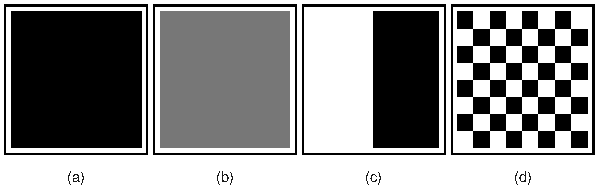
\includegraphics[width=\linewidth]{figs/checkerboard.pdf}
		\begin{tabular}{l | c c c} 
		\textbf{City} & $H(Y)$ & $I(X,Y)$ & $J(X,Y)$ \\
		\hline
		(a) & $0$        & $0$        & $0$\\
		(b) & $\log 2$ & $0$        & $0$\\
		(c) & $\log 2$ & $\log 2$ & $\frac{1}{7} \log 2$\\
		(d) & $\log 2$ & $\log 2$ & $\log 2$
		\end{tabular}
		\caption{
			\emph{(Top)}: Schematic cities illustrating three dimensions of segregation. 
			City (a) lacks global diversity, while cities (b)-(d) are maximally globally diverse. 
			City (b) is perfectly spatially even, whereas cities (c) and (d) are maximally uneven. 
			City (c) has lower spatial exposure than city (d), since a typical small area of (c) (shown in highlight) is monoracial.
			In contrast, a typical small neighborhood of (d) has multiple contact points between racially distinct areas. 
			\emph{(Bottom)}: Information measures of each city. Entropy separates cities (a) and (b); mutual information separates (b) and (c), and mean local information separates (c) and (d). 
		} \label{fig:checkerboard}
	\end{figure}
\subsection*{Mutual Information and Spatial Evenness}
	Local-to-global measures depend on comparisons between properties encoded by the local compositions $p(Y|x)$ and the global composition $p(Y)$. 
	When each of the compositions $p(Y|x)$ is the same as $p(Y)$, the city is perfectly spatially even -- every racial group is represented at each location in proportion to their presence in the city overall. 
	When the local compositions $p(Y|x)$ differ from $p(Y)$, the city is spatially uneven. 
	We can measure spatial evenness as the average difference between local and global compositions: 
	\begin{equation}
		I(X,Y) = \E_X[D[p(Y|X)\|p(Y)]\;.
	\end{equation}
	The operator $\E_X$ denotes average or expectation with respect to the probability distribution of $X$. 
	The quantity $I(X,Y)$ is called the \emph{mutual information} in information theory \cite{Cover1991,Csiszzr2004,Bettencourt2015}.  
	When all groups are evenly distributed, such as in Figure \ref{fig:checkerboard}(b), each location has the same composition as the global composition, and $I(X,Y) = 0$. 
	On the other hand, $I(X,Y)$ achieves its maximum value of $\log \abs{\mathcal{Y}}$ when every location is monogroup, such as in Figure \ref{fig:checkerboard}(c). 

\subsection*{Local Information and Spatial Complexity}
	
	Global and local-to-global measures can illuminate important high-level urban structure, but miss an important class of phenomena. 
	The model two-race cities (c) and (d) in Figure \ref{fig:checkerboard} each have the same values of $H(Y)$ and $I(X,Y)$. 
	City (c), however, has a single dividing line of racial separation, while city (d) has smaller pockets of racial distinctiveness. 
	In sociology or urban planning, this may be the difference between metastasized segregation and healthy variation. 
	The difference is intrinsically local: while the typical small neighborhood of city (c) is monoracial, the typical small neighborhood of (d) contains multiple contact points between different racial groups. 
 
	To measure local variation, imagine segmenting the city into a grid of small cells. 
	The \emph{local mutual information} in the cell $B$ is the mutual information between $X$ and $Y$, restricted to $B$:
	\begin{equation*}
		I(X,Y | X \in B) = \E_{X|X \in B}[D[p(Y|X,X\in B)\|p(Y|X\in B)]\;.
	\end{equation*}
	The local information can be interpreted as the degree of change in demographics one would observe if one started in $B$ and then walked a small distance away. 

	If we regard the data as a discretization of a smooth probability field, then it is possible to show using arguments from information geometry \cite{Amari2000} that the local information in a cell $B$ of radius $r$ is an approximation of the Fisher information $\mathcal{J}$:
	\begin{equation}
		I(X,Y|X \in B) \cong \frac{r^2}{4} \text{tr } \mathcal{J}_Y(x)\;, \label{eq:fisher_approx}
	\end{equation}
	where $[\mathcal{J}_Y(x)]_{ij} = \E_Y[-\partial_{x_i} \partial_{x_j} \log p(Y|x)]$ is the Fisher information matrix and $\text{tr } \mathcal{J}_Y(x)$ is the sum of its eigenvalues. 

	The \emph{mean local information} measures the average local variation in group composition across the entire city:  
	\begin{equation}
		J(X,Y) = \E_B[I(X,Y|X \in B)]\;.
	\end{equation}
	Figure \ref{fig:Atlanta_philly} shows the computation of $J(X,Y)$ for Atlanta and Philadelphia. While the two cities have similar entropies $H(Y)$ and mutual informations $I(X,Y)$, their spatial structures are substantially different. Atlanta is characterized by a stark North-South divide between white and black residents. As a result, there are many areas in Atlanta where the local information is near $0$. These are areas in which one can walk for $1km$ or more without experiencing significant demographic change. Such areas are relatively rare in Philadelphia, which consists of a finer patchwork of demographically varying neighborhoods. Philadelphia therefore has a higher value of mean local information, reflecting greater spatial complexity in demographic variation. 


	\begin{figure}
			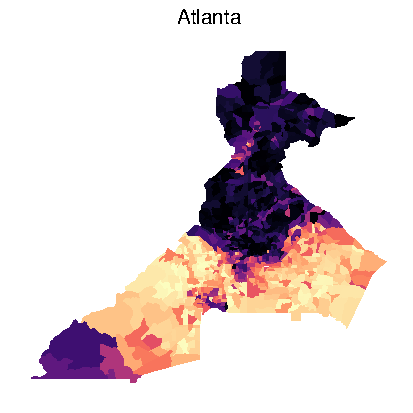
\includegraphics[width = .5\linewidth]{figs/Atlanta_percent_black.pdf}
			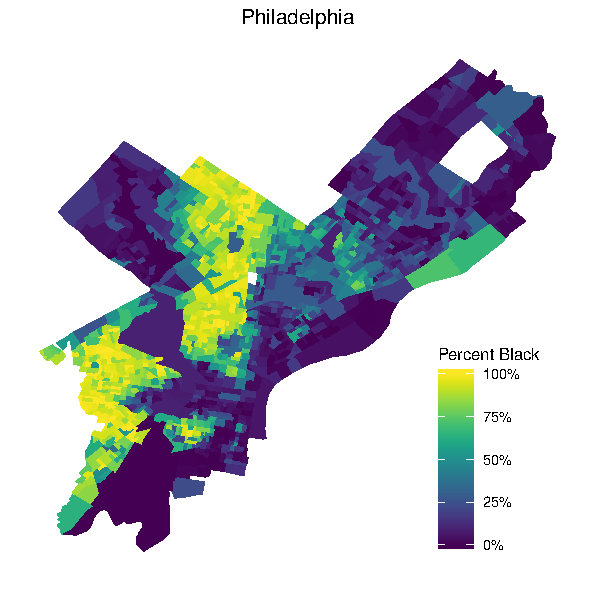
\includegraphics[width = .5\linewidth]{figs/Philadelphia_percent_black.pdf} \\
			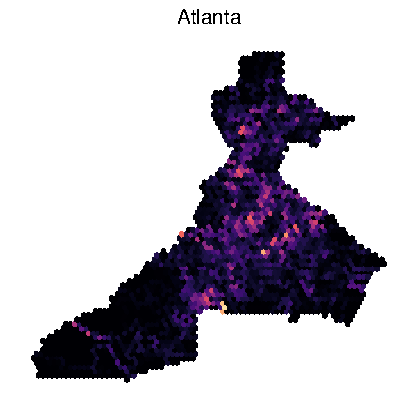
\includegraphics[width = .5\linewidth]{figs/Atlanta_grid.pdf} 
			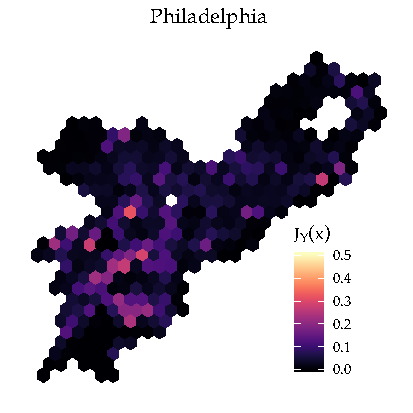
\includegraphics[width = .5\linewidth]{figs/Philadelphia_grid.pdf} \\

			\centering
			\begin{tabular}{l | c c c c}
				\bfseries City & Percent Black & $H(Y)$ & $I(X,Y)$ & $J(X,Y)$  \\\hline
				\csvreader[late after line=\\]{figs/comparative_summary.csv}{}
				{\csvcoli & \csvcolii & \csvcoliii & \csvcoliv & \csvcolv}
			\end{tabular}

			\caption{
				(\emph{Top}): Percentage of black residents. 
				(\emph{Middle}): Hexgrid of spatial resolution 1km imposed over each city. Within each hex $B$ we compute the local information local information $J_Y(B) = I(X,Y | X \in B)$. 
				(\emph{Bottom}): Numerical summary including entropy, mutual information, and mean local information. 
			} \label{fig:Atlanta_philly}
	\end{figure}

\subsection*{Separation Profiles in the US}
	
	We can view Atlanta and Philadelphia in broader context by comparing $I(X,Y)$ and $J(X,Y)$ across a range of American cities in Figure \ref{fig:mutual_fisher}. 
	For each city, we computed $J(X,Y)$ using a 1km hexgrid and the racial categories $\mathcal{Y} = \{\text{Asian}, \text{ Black}, \text{ Hispanic}, \text{ Other}, \text{ White}\}$. 
	The mutual information and local information sort cities into three primary classes. 
	Those toward the bottom left have low $I(X,Y)$ and therefore display relatively little spatial variation. 
	Cities become more unevenly distributed as we move rightward. 
	Those toward the bottom right, such as Atlanta and Detroit, are both highly uneven and have little local variation. 
	These cities are highly segregated, with large, starkly separated monoracial regions. 
	In contrast, cities toward the top right like Philadelphia and New York are more complex patchworks of smaller, ethnically distinct subregions.  

	\begin{figure}
		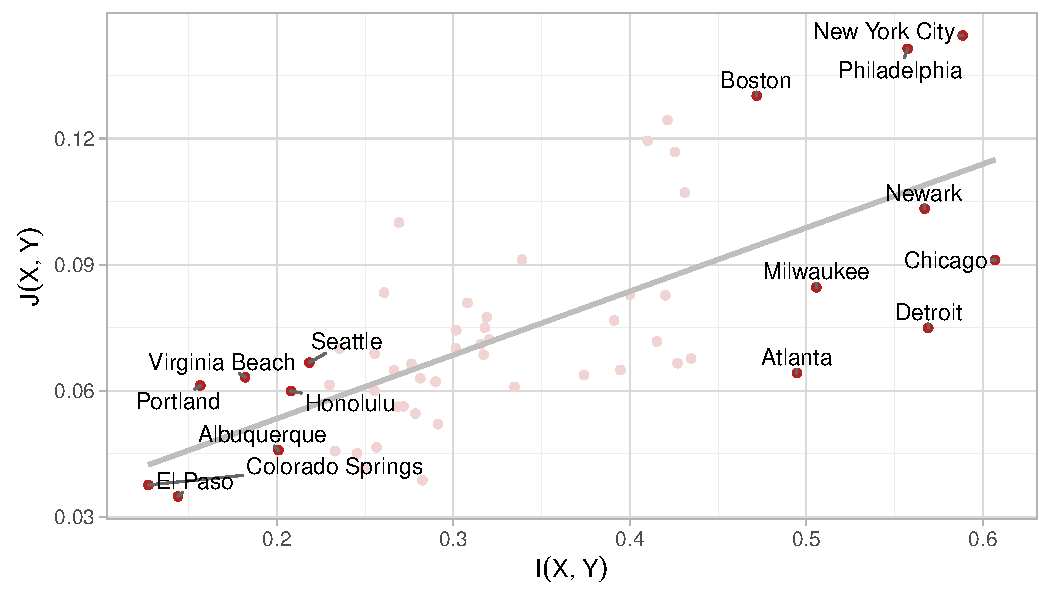
\includegraphics[width=\linewidth]{figs/mutual_fisher.pdf}
		\caption{
			Comparative global segregation measures in major U.S. cities, measured using racial categories $\mathcal{Y} = \{\text{Asian}, \text{ Black}, \text{ Hispanic}, \text{ Other}, \text{ White}\}$. 
			A hexgrid of spatial resolution $r = 1$km was for the computation of $J(X,Y)$. The grey line is the linear least-squares regression line provided as a visual aid. 
		} \label{fig:mutual_fisher}
	\end{figure}

\subsection*{Identifying Sociospatial Structure} 
	The measures $H(Y)$, $I(X,Y)$, and $J(X,Y)$ quantify the presence of global, local-global, and purely local sociospatial structure. We can also use information methods to identify and visualize that structure directly. While approaches exist to this problem,\footnote{For three, see \cite{Logan2011}} these approaches tend to conceptualize this structure in terms of monoracial subregions. In practice, however, there may be coherent biracial or multiracial patterns in space. Information methods define a useful approach. 
	\begin{figure}

		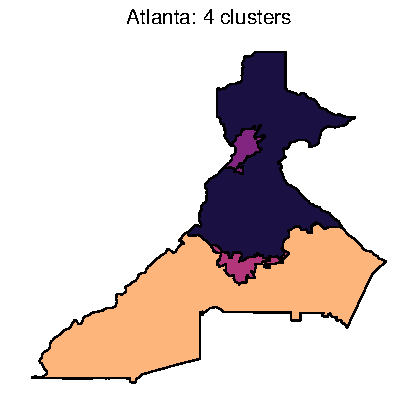
\includegraphics[width = .5\linewidth]{figs/Atlanta_clusters_binary_4.pdf} 
		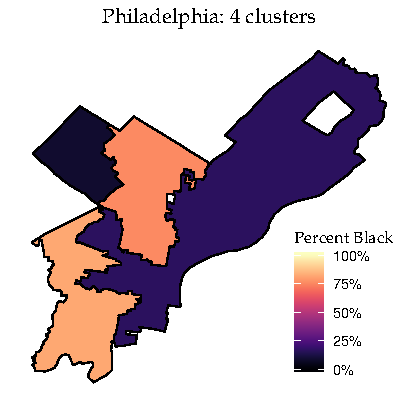
\includegraphics[width = .5\linewidth]{figs/Philadelphia_clusters_binary_4.pdf} \\
		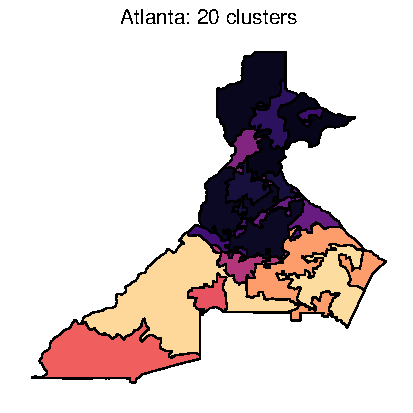
\includegraphics[width = .5\linewidth]{figs/Atlanta_clusters_binary_20.pdf}
		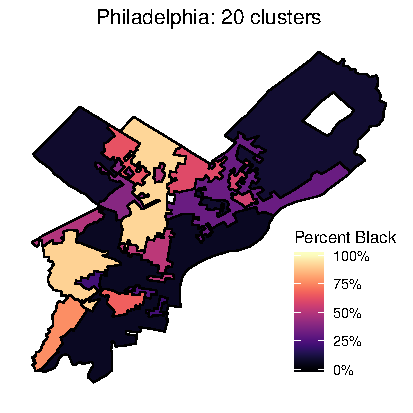
\includegraphics[width = .5\linewidth]{figs/Philadelphia_clusters_binary_20.pdf} \\
		
		\centering
		\begin{tabular}{l | c c c}
			\bfseries City  & $I(C_4, Y)$ & $I(C_{20},Y)$ & $I(X,Y)$ \\\hline
			\csvreader[late after line=\\]{figs/clustering_summary.csv}{}
			{\csvcoli & \csvcoliii & \csvcoliv & \csvcolii}
		\end{tabular}
		\caption{
			\emph{(Top)}:Example clusterings in Atlanta and Philadelphia using \eqref{eq:cluster_opt}, using $4$ and $20$ clusters. 
			\emph{(Bottom)}: Comparison of information content of clusterings and total mutual information in each city. 
		} \label{fig:clusterings}
	\end{figure}
	Let $C$ be a grouping of the locations $X$. Mathematically, $C$ is a random variable with the property that that $H(C|X) = 0$. The chain rule of information\footnote{See \cite{Cover1991}} implies that 
	\begin{equation}
		I(X,Y) = \underbrace{I(C,Y)}_{\text{between-group}} + \underbrace{I(X,Y|C)}_{\text{within-group}}. \label{eq:chain_rule}
	\end{equation}
	Analogous to sum-of-squares maximization in statistics, we wish to maximize $I(C,Y)$ subject to a fixed number of clusters, an approach popularized by \cite{Dhillon2003,Banerjee2005}. In full generality, this is a challenging discrete optimization problem that may not be computationally tractable. Additionally, for interpretability, should be clustered together only when they are adjacent in space. To handle these two problems, we use a greedy algorithm based on agglomerative clustering. At stage of the algorithm, we consider the problem of choosing a pair of locales $\{i*, j*\}$ such that aggregating them minimizes information loss. We quantify the loss as follows. The mutual information over the full complement $\mathcal{K}$ of locales may be written: 
	\begin{align*}
	 	I(X,Y) &= \sum_{k \in \mathcal{K}} p(X = k) D[p(Y|X = k\|p(Y)] 
	\end{align*} 
	The contribution of locale $k$ to this sum is 
	\begin{align*}
		I_{k}(X,Y) &= p(X = k)D[p(Y|X = k)\|p(Y)]. 
	\end{align*}
	If we replace $i$ and $j$ with an aggregated locale $i\cup j$, the aggregated locale's contribution to the mutual information is 
	\begin{align*}
		I_{i\cup j}(X,Y) = p(X \in \{i,j\}) D[p(Y|X \in \{i,j\}) \| p(Y)]\;.
	\end{align*}
	The loss associated with aggregating $i$ and $j$ is the difference between their individual contributions and the aggregated contribution of $i\cup j$:
	\begin{align*}
		d(i,j) = I_{i}(X,Y) + I_{j}(X,Y) - I_{i \cup j}(X,Y).  
	\end{align*}
	The function $d$ may be regarded as a similarity measure. It satisfies $d(i,j) = 0$ if and only if $p(Y|X = i) = p(Y|X = j)$; i.e. the demographic profiles of locations $i$ and $j$ are identical. It is also symmetric in $i$ and $j$. We can use it to motivate a form of agglomerative hierarchical clustering, where at each phase of the algorithm we compute 
	\begin{equation}
		(i^*, j^*) = \argmin_{i \text{ neighbors } j} \; d(i,j)\; \label{eq:cluster_opt}
	\end{equation}
	and combine $i^*$ and $j^*$ into a single new locale, repeating until only a specified number $n$ locales remain. 
	Equation \eqref{eq:cluster_opt} defines \emph{spatially constrained, information-maximizing agglomerative clustering}. 
	Since the algorithm is greedy, it possesses no guarantees of optimality, but in practice its performance leads to intuitive, demographically-coherent regions. 
	The resulting regions may be viewed as coarse-grainings of the spatial structure, which emphasize high-level patterns and abstract away details. 

	Figure \ref{fig:clusterings} demonstrates this information-maximizing agglomerative clustering for Atlanta and Philadelphia, using 4 and 20 clusters. In Atlanta, the algorithm immediately highlights the prominent North-South divide, while in Philadelphia it segments two predominantly Black regions on either side of the Schuykill river from the rest of the city. As we allow the algorithm to use progressively more clusters, it highlights progressively more subtle patterns of variation. Strikingly, in Atlanta just 4 clusters are sufficient to capture 0.27 nats of information, where in Philadelphia 20 clusters are needed. Philadelphia has more complex sociospatial trends: compared to Atlanta, more complex models are necessary to model it to a similar degree of accuracy. 
	
	
	\begin{figure}
		\centering
			% \begin{subfigure}[b]{0.45\linewidth}
			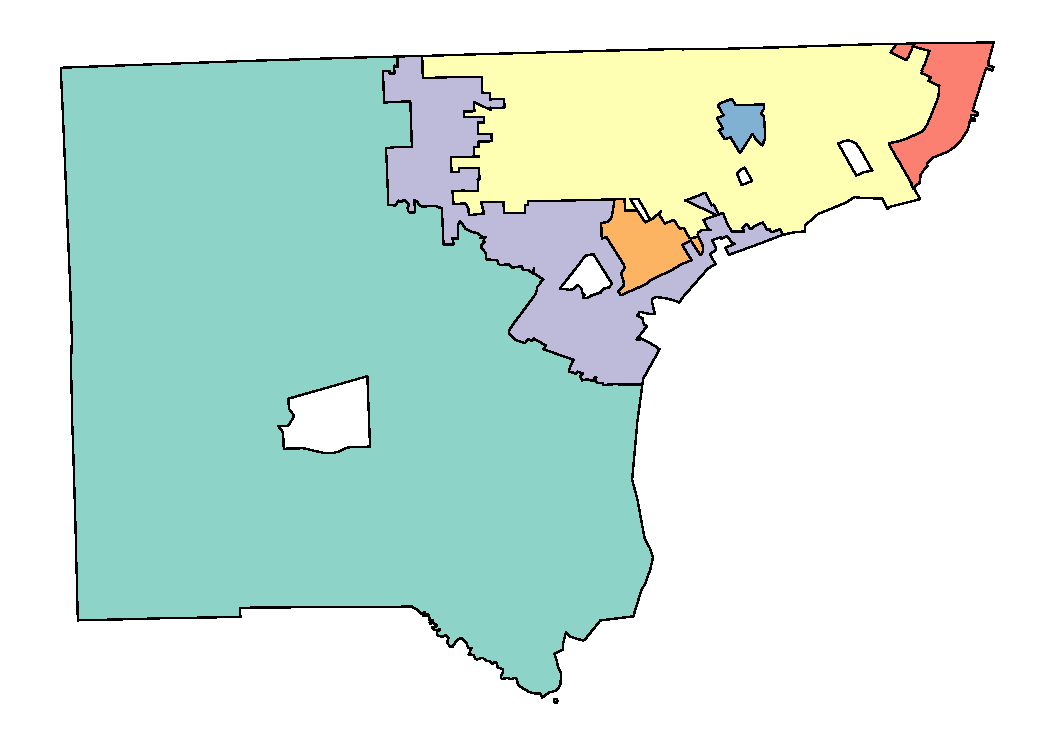
\includegraphics[width = .5\linewidth]{figs/example_cluster_map.pdf}
			% \caption{} \label{subfig:detroit_map}
			% \end{subfigure}
			% \begin{subfigure}[b]{0.45\linewidth}
			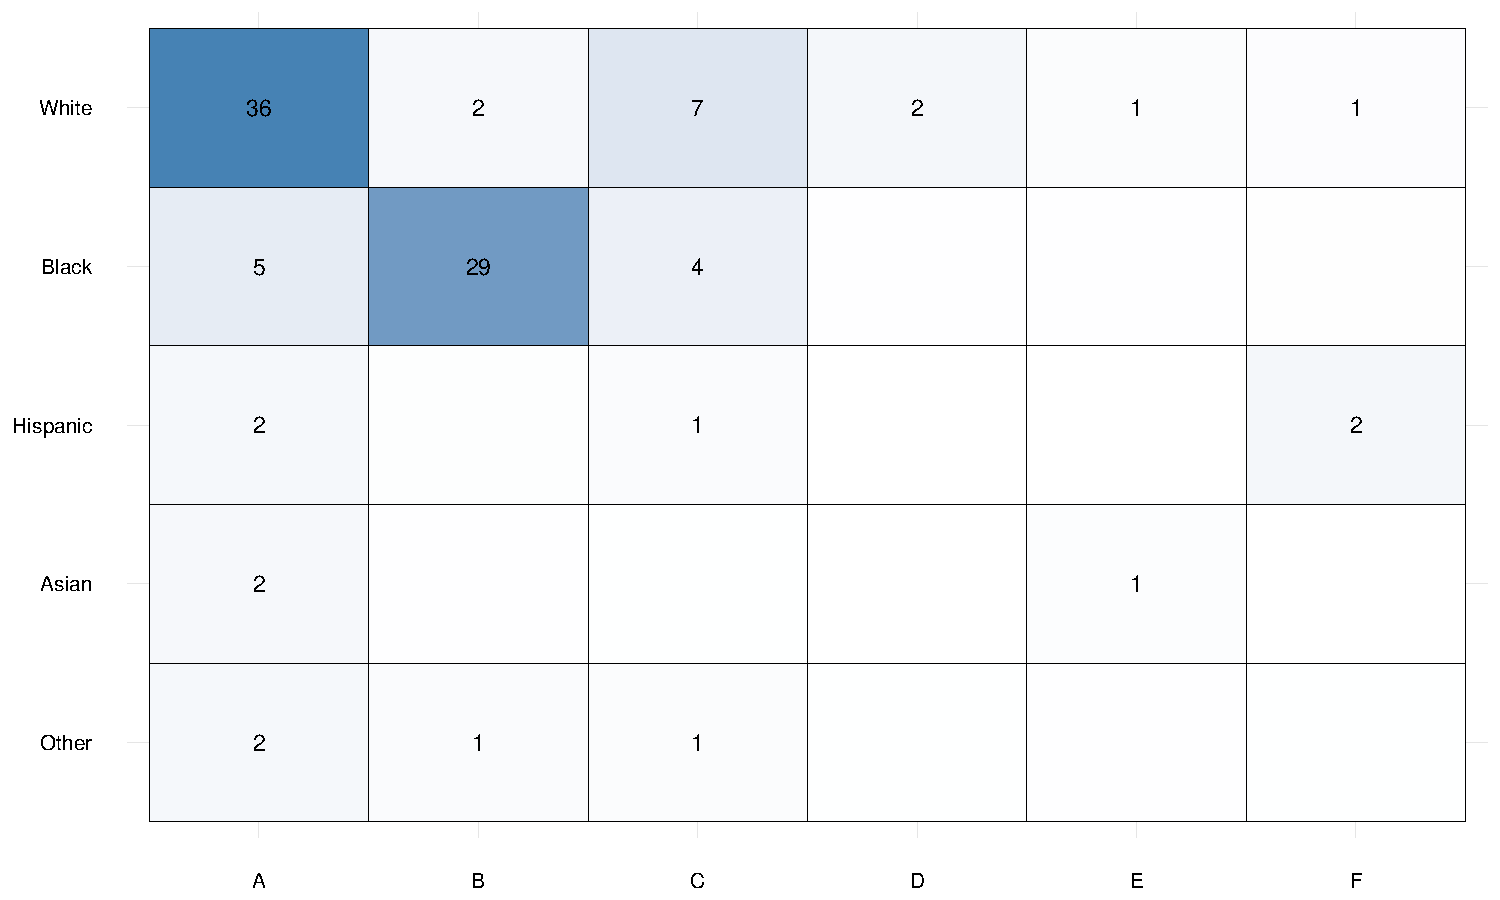
\includegraphics[width = .45\linewidth]{figs/example_clusters_detailed.pdf}
			% \caption{} \label{subfig:detroit_groups}
			% \end{subfigure}
			\caption{
				Multigroup sociospatial structure in Detroit. 
				\emph{(Left)}: Map of six clusters. 
				\emph{(Right)}: Joint distribution of demographics and clusters. 
				Shadings reflect population proportions within clusters. 
				Numerical labels give raw population proportions; for example, 29\% of the population is Black and resides in cluster B. 
				Detroit has $H(Y) = 1.12$, $I(X,Y) = 0.57$, and $J(X,Y) = 0.08$. 
				This clustering captures $I(C_6,Y) = 0.36$ nats of information.
			} \label{fig:detroit}
	\end{figure}

	Information-maximizing agglomerative clustering also applies to multigroup analysis.  Figure \ref{fig:detroit} shows a multigroup clustering in Detroit and the surrounding Wayne County. The prominent clusters A and B reflect the primary white/black division in the city, with A representing the white suburbs and B the denser black inner city. Cluster C is interpretable as a transitional area between these two populations, with both white and black residents represented. Cluster D coincides with the historically distinct, predominantly white town of Grosse Pointe. Cluster E coincides with the city of Hamtramck, whose history has been shaped by high levels of immigration from Europe and Asia. Finally, Cluster F coincides with the Hispanic neighborhood Mexicantown. 

	This technique also enables novel quantitative methods for studying traditional concerns in segregation studies. According to \cite{Massey1988}, ``\emph{concentration} refers to the degree of a group's agglomeration in urban space.'' The concept of concentration invites us to consider the composition and density of each cluster. For example, whites make up 70\% of ``their'' cluster A, while black residents make up 86\% of ``their'' cluster B. Cluster B is also more densely populated than Cluster A: it contains 34\% of Wayne County's population, but just 19\% of the analyzed geographic area, making it more than twice as dense as Cluster A. Thus, in and around Detroit, black neighborhoods tend to be both more racially homogeneous and more densely packed in urban space than white ones. We can also learn about pairwise group exposure. For example, from Figure  \ref{fig:detroit}, Asian residents tend to be found alongside white residents, but more rarely alongside black or Hispanic residents. Hispanic residents tend to group in Mexicantown and in predominantly white neighborhoods, but not black ones.

\subsection*{Local Information and Spatial Complexity}
	The mean local information measures the number and character of spatial transitions between demographically distinct regions. When there are many, we would expect that information-maximizing agglomerative clustering would require more clusters to capture similar amounts of information. We can empirically quantify the relationship between $J(X,Y)$ and the performance of information-maximizing clustering as follows. Consider the between-groups information $I(C_n,Y)$ plotted as a function of the number $n$ of clusters. The result is a curve reflecting how information scales at varying levels of aggregation, as shown in Figure \ref{fig:AUC} shows examples of these curves for Atlanta, Detroit, and Philadelphia. 

	The area under these curves is a measure of how early information is ``captured'' by the clustering. When the AUC is high, small numbers of clusters suffice to capture most of the information. Atlanta and Detroit illustrate this case, as both can be starkly divided into monolithic Black and non-Black regions. In Philadelphia, in contrast, the AUC is lower and more complicated models are necessary, as was illustrated in \ref{fig:clusterings}. The explicit formula for the AUC is
	\begin{equation}
		AUC = \frac{1}{I(X,Y) \log N} \sum_{n=1}^N I(C_n, Y) \log \frac{n+1}{n}, \label{eq:AUC_formula}
	\end{equation}
	To show the relationship between $J(X,Y)$, we conduct a simple linear least-squares fit of the form
		\begin{equation*}
			AUC \approx m_1H(Y) + m_2I(X,Y) + m_3J(X,Y) + b\;.
		\end{equation*}
	Figure \ref{fig:regression} gives the summary table for this fit. Collectively, the three information measures suffice to explain an adjusted 75\% of the variation in the AUC, showing that the AUC is highly dependent on the information structure of sociospatial variation. The signs of the coefficients are also interpretable. The largest magnitude by far is the coefficient of $I(X,Y)$; all else equal, clustering is more effective when groups are distributed unevenly. The negative sign on the coefficient of the mean local information $J(X,Y)$ shows that for fixed $H(Y)$ and $I(X,Y)$, higher values of $J(X,Y)$ (more sociospatial complexity) indicate cities that are harder to capture using coarse-grained models. 
	\begin{figure} 
			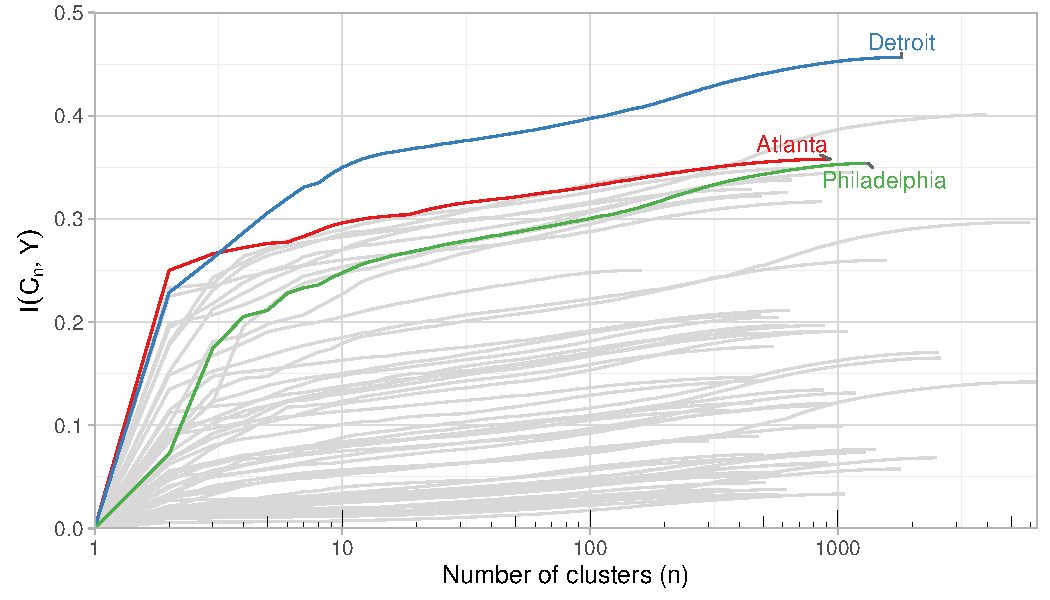
\includegraphics[width=\linewidth]{figs/binary_loss_curves.pdf}

			\vspace{0.5cm}

			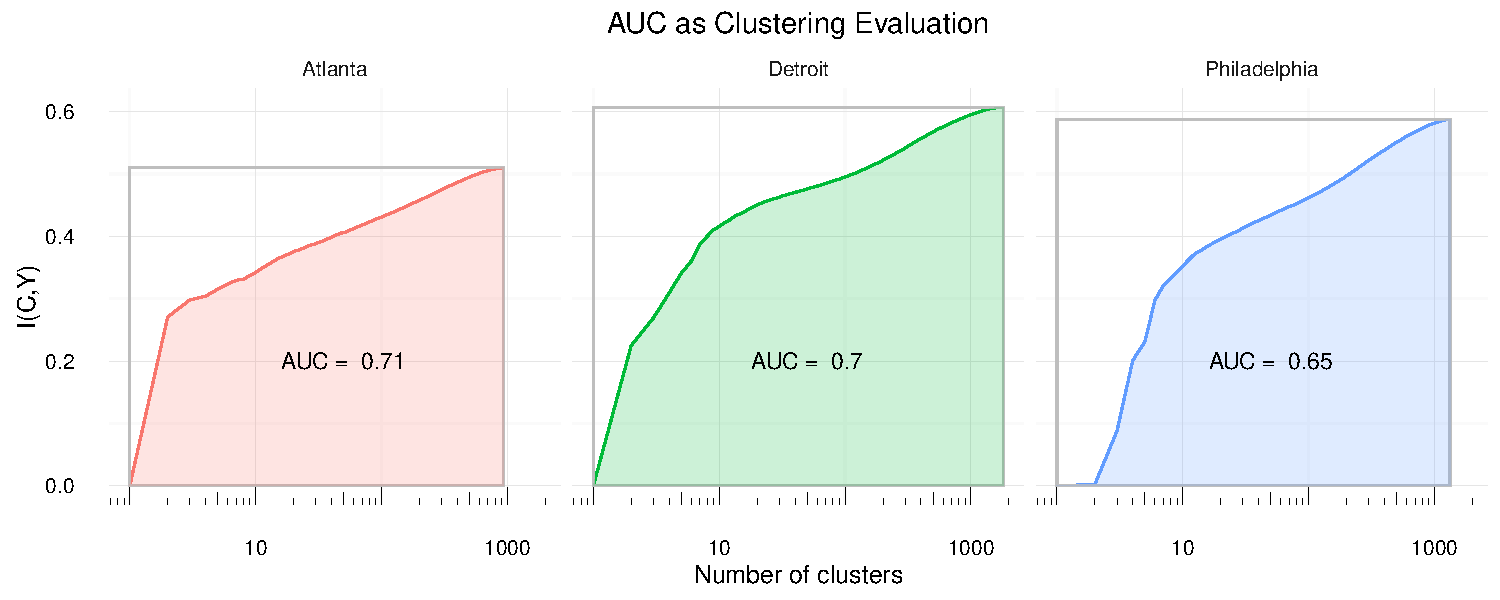
\includegraphics[width=\linewidth]{figs/AUC_illustration.pdf}
			\caption{
				\emph{(Top)}: Hierarchical scaling of information for Black/Non-black segregation patterns in major U.S. cities.  
				Each curve is a complexity profile for sociospatial structure in a city. 
				Atlanta and Detroit's curves rise sharply and then level off, indicating that relatively few clusters suffice to express most of the sociospatial structure. 
				Philadelphia's curve rises more slowly, indicating the need for more complex models. 
				\emph{(Bottom)}:
				Complexity quantification using the area under the curve (AUC) for $\mathcal{Y} = \{\text{Black }, \text{Non-Black}\}$, computed according to the formula \eqref{eq:AUC_formula}. 
				The AUC is the proportion of the bounding rectangle contained within the shaded region. 
				Lower values of the AUC correspond to more complex structure. 
			} \label{fig:AUC}
	\end{figure}
	
	\begin{figure}
		\centering
		\input{figs/adjusted_regression.txt}
		\caption{
			Regression of the AUC computed by \eqref{eq:AUC_formula} on the information measures $H(Y)$, $I(X,Y)$, and $J(X,Y)$. 
			95\% confidence intervals for each of the determined coefficients are shown in parentheses. 
			The three information measures jointly explain an adjusted 75\% of the variation in the AUC. 
		}\label{fig:regression}
	\end{figure}

\section*{Discussion}
	
	\subsection*{Local Information as a Complexity Measure}
		The local information $J(X,Y)$ is a measure of spatial exposure contextualized by the mutual information. It can also be viewed as a measure of \emph{intrinsic sociospatial complexity}. Cities with high mean local information, such as Philadelphia, have more complex spatial structure than those with low mean local information such as Atlanta. Urban complexity has been a lively topic of interest at the intersection of physics and urban planning. Physically, the complexity of cities can be viewed as a rough measure of the complexity of theories needed to explain their structure and dynamics \cite{Bettencourt2015}. From a planning perspective, the complexity of land use was famously theorized by Jane Jacobs \cite{Jacobs1992} to be a driver of the health of neighborhoods. This theory has received preliminary empirical support \cite{DeNadai2016a}, with more tests no doubt to come. The local information can capture local variations in land use as well as demographics. We hope that this measure will serve as a useful tool for scholars of urban spatial complexity.  
	\subsection*{Local Information as a Complexity Measure}
		A major challenge for information theory in urban science is the development of principled dynamical models that can explain variations in observed information measures across cities \cite{Batty2014a}. One approach to this challenge is to observe how information changes over time at varying scales. On the timescale of decades, information measures may be used to analyze the evolution of the evolving sociospatial structure of cities. Information-maximizing agglomerative clustering could then be used to cluster coherent regions in time as well as space, enabling a view of shifting demographic boundaries.

		Another avenue of exploration is on the much shorter timescale of daily mobility. Many adults spend less than half of their waking hours at home \cite{BureauofLaborStati2014}, indicating that residential segregation is only a partial characterization of city-wide diversity. Fortunately, our ability to learn about daily patterns of human mobility is progressing at a rapid pace. Recent years have seen an enormous increase in the use of mobile devices, allowing the passive collection of digital traces. These traces can be processed, analyzed, and validated to derive insight into daily activity patterns \cite{Widhalm2015,Yang,Jiang2013,Jiang2012c}. By combining these traces with residential demographics, it is possible to estimate flows of different demographic groups throughout the city on a daily basis. 
	\subsection*{Spatial Preprocessing}
		The measures we have developed use their data (provided by the Census) as an unbiased approximation of the true distribution of racial groups across locations. This approach has two limitations. First, the demarcations of Census areal units are to some extent arbitrary: changing them would not change the underlying demographic phenomena, but may change the values of the mutual information or local information \cite{Openshaw1981}. Second, cities are anisotropic: two neighborhoods may be no more than 50 meters away, but if they are separated by a river, they may be functionally ``farther'' from each other than two other neighborhoods 500m apart. An approach to address both criticisms is to spatially preprocess the data using a smoothing kernel, as demonstrated in \cite{Roberto2015} for the case of the mutual information. Further experiments on the numerical impact of MAUP and anisotropy are called for in order to determine whether the benefit of preprocessing justifies the additional computational costs of this procedure.   


\matmethods{
		\subsection*{Data Access}
		All data used in this study are freely available from the U.S. Census. The \texttt{R} packages \texttt{acs} and \texttt{tigris} were used to programmatically download demographics and geographic shapefiles, respectively. All demographic data is from the Five-Year Estimates of the 2014 American Community Survey, Table B03002. 
		\subsection*{Software Repositories}
			We are pleased to make available two software repositories accompanying this analysis. Package \texttt{compx} for the \texttt{R} programming language implements computation of the information measures $H(Y)$, $I(X,Y)$, and $J(X,Y)$, as well as a method for information-theoretic clustering. Access \texttt{compx} at \texttt{https://github.com/PhilChodrow/compx}. 
			
			The analysis repository for this project includes data acquisition and processing; core computations; and figure generation. We hope that this repository will provide useful examples of how to use \texttt{compx} for others aiming to replicate and extend our results. Download the project files at \texttt{https://github.com/PhilChodrow/spatial\_complexity}. 
			  
		\subsection*{Delimiting Cities} 
		The delimiting of cities based on non-arbitrary population densities or natural boundaries is an area of active discussion in urban planning. For recent advances, see \cite{Rozenfeld2008,Rozenfeld2011}. W took a simple approach for the purposes of this study. For each city considered, we analyzed the region composed of all (and only those) counties in which some or all of the city's municipal boundaries lie. For example, our region corresponding to Atlanta consists of Fulton and Dekalb Counties, our region corresponding to Philadelphia consists of Philadelphia County, and the region corresponding to Detroit consists of Wayne County. For independent cities such as Baltimore and Washington D.C., the region of analysis consists simply of the municipal city boundaries. 
		\subsection*{Aggregation of Racial Categories} 
		The data provided by Table B03002 contains categories corresponding to two options for ethnicity (Hispanic or Latino, Not Hispanic or Latino) and nine corresponding to race, giving a total of 18 cross-tabulated categories. For the purposes of analysis, we aggregated these into just five categories, \{\text{Asian}, \text{Black}, \text{Hispanic}, \text{Other}, \text{White}\}. The correspondence used is given in the GitHub repository \texttt{PhilChodrow/spatial\_complexity} linked above, under \texttt{assumptions/race\_lookup.csv}. 
		\subsection*{Analysis and Visualization} 
		All analysis and visualization was conducted in the \texttt{R} statistical programming language. We used \cite{Bivand2014b,Bivand2014a,Bivand2014} for geographic analysis, and \cite{Wickham} for visualization.
}

\showmatmethods{} % Display the Materials and Methods section

\acknow{P.C. is grateful to Marta C. Gonz\'{a}lez for helpful discussion, and to MIT-Saudi Arabia...}

\showacknow{} % Display the acknowledgments section

% \pnasbreak splits and balances the columns before the references.
% Uncomment \pnasbreak to view the references in the PNAS-style
% If you see unexpected formatting errors, try commenting out \pnasbreak
% as it can run into problems with floats and footnotes on the final page.
% \pnasbreak

% \nocite{Bettencourt2013}

% Bibliography
\bibliography{/Users/phil/bibs/library.bib}

\end{document}